\documentclass[sigconf,anonymous]{acmart}

\usepackage{booktabs} % For formal tables
\usepackage{enumitem}
\usepackage{natbib}
\usepackage{mathtools}
\usepackage{amssymb}
\usepackage{amsthm}
\citestyle{acmnumeric}


% Copyright
%\setcopyright{none}
%\setcopyright{acmcopyright}
%\setcopyright{acmlicensed}
\setcopyright{rightsretained}
%\setcopyright{usgov}
%\setcopyright{usgovmixed}
%\setcopyright{cagov}
%\setcopyright{cagovmixed}

% CFP: http://esec-fse17.uni-paderborn.de/call_for_papers.php
% Template: http://www.acm.org/publications/proceedings-template

% DOI
\acmDOI{10.475/123_4}

% ISBN
\acmISBN{123-4567-24-567/08/06}

%Conference
\acmConference[ESEC/FSE'17]{ACM conference}{September 2017}{El
	Paderborn, Germany} 
\acmYear{2017}
\copyrightyear{2017}

\acmPrice{15.00}


\begin{document}
%\title{Got To Go}

\title{Quantifying Security Context Factors in Software Development}


\author{Patrick Morrison}
\affiliation{%
	\institution{Department of Computer Science}
	\streetaddress{North Carolina State University}
	\city{Raleigh}
	\state{North Carolina} 
	%\postcode{43017-6221}
}
\email{pjmorris@ncsu.edu}

% Asked to be left off of paper, pending closer review
%\author{Jonathan W. Stallings}
%\affiliation{%
%	\institution{Department of Statistics}
%	\streetaddress{North Carolina State University}
%	\city{Raleigh}
%	\state{North Carolina} 
%	%\postcode{43017-6221}
%}
%\email{jwstallings@ncsu.edu}

\author{Laurie Williams}

\affiliation{%
	\institution{Department of Computer Science}
	\streetaddress{North Carolina State University}
	\city{Raleigh}
	\state{North Carolina} 
	%\postcode{43017-6221}
}
\email{williams@csc.ncsu.edu}

	
\begin{abstract}
\label{sec:abstract}
Context: Researchers and practitioners have proposed and evaluated many practices for measuring and improving software security during software development. However, assessing the effectiveness of security practices requires measuring not only the practices and their effects on software, but the software's characteristics and the context in which the software is used. 

Goal:  \textit{The goal of this research is to support researchers and practitioners in measuring the effect of security practice use on software vulnerabilities by building and evaluating an explanatory model for software development security practice use.} 

Method: In this work, we develop a model hypothesizing relationships between security outcomes, adherence to security practices, software context factors, and environmental context factors.  We evaluate the model quantitatively, using two existing datasets: The National Vulnerability Database (NVD), containing 79,533 vulnerabilities, and the Core Infrastructure Initiative (CII) census dataset of 428 security-critical projects.  

Results: As measured in our data, both environmental context factors and software characteristics had strong correlations with security outcomes. The NVD case study results agreed with previous research suggesting that software security has improved over the last decade, as measured by decreasing CVSS scores and increasing access complexity required of attackers. The CII case study results agreed with previous research suggesting that team size and effort, and code size, are among the most significant influences on vulnerabilities. 
Conclusion: The developed model and results from the two case studies offer a guide to the metrics suitable for prioritizing management of software context factors and security outcomes. 


\end{abstract}

%\ccsdesc[500]{Keywords got to go~Redundancy}
%\ccsdesc[300]{Computer systems %organization~Redundancy}
%\ccsdesc{Computer systems organization~Robotics}
%\ccsdesc[100]{Networks~Network reliability}

% We no longer use \terms command
%\terms{Theory}

%\keywords{ACM proceedings, \LaTeX, text tagging}

\maketitle

\section{Introduction}
\label{sec:intro}
In February 2017, security researchers discovered a programming bug in an HTML parser at Cloudflare\footnote{https://blog.cloudflare.com/incident-report-on-memory-leak-caused-by-cloudflare-parser-bug/}. The parser was sending decrypted encryption keys and passwords along with ordinary web requests, resulting in unencrypted sensitive data being cached across the Internet. While the programming bug, now known as `Cloudbleed'~\footnote{https://blog.cloudflare.com/quantifying-the-impact-of-cloudbleed}, was on a single line of code, the bug had widespread effects because of the code's context, running on many servers, and sending sensitive results to many clients. The example of Cloudbleed suggests that software development teams must consider software's environment and data as well as the technical characteristics of their software when evaluating their software's security. 

The IEEE defines security~\cite{ieee1990glossary} as 'all aspects related to defining, achieving, and maintaining confidentiality, integrity, availability, non-repudiation, accountability, authenticity, and reliability of a system.' Several lists of practices for specifying how a development team defines, achieves, and maintains the security properties listed above (confidentiality, integrity, availability, non-repudiation, accountability, authenticity, and reliability) in the software the team produces have been published. Example lists include the Building Security in Maturity Model ~\cite{mcgraw2006software}
(BSIMM), the Microsoft Security Development Lifecycle ~\cite{howard2009security} (SDL), the Software Assurance Forum for Excellence in Code~\cite{simpson2013fundamental} (SAFECode), and the Open Web Application Security Project (OWASP) Software Security Assurance Process ~\cite{martinez2014ssap} (SSAP). While defining how software will support the various security properties lies within the control of the development team, the observed security outcomes also depend on factors outside of the development team's direct control. Two pieces of software may have similar technical characteristics (e.g. same language, same size) but different security outcomes as a consequence of the uses to which the software is put. For example, between a game level editor and a database system of similar source code size, the database system managing credit card data may be more prone to attack, and to have publicly reported vulnerabilities~\footnote{Following Krsul~\cite{krsul1998software} and Ozment~\cite{ozment2007vulnerability}, we define a vulnerability as “an instance of a mistake in the specification, development, or configuration of software such that its execution can violate the explicit or implicit security policy.}, than the game level editor managing custom game levels. 

Multiple software technical and process characteristics contribute to the potential for software vulnerabilities. For example, code size ~\cite{alhazmi2007measuring}, code churn ~\cite{shin2011evaluating,meneely2013when}, and language ~\cite{ray2014a} have been correlated with vulnerabilities. Similarly, multiple software usage characteristics, for example, access to sensitive data~\footnote{http://heartbleed.com/}, management of financial information~\cite{harris2014for}, and the presence of a piece of software on large numbers of machines~\footnote{http://www.cert.org/historical/advisories/CA-2001-19.cfm} have been correlated with vulnerabilities. Finally, the practices a development team chooses to apply, and the degree to which they adhere to those practices, affects the number and kind of vulnerabilities in their software. As an example of a specific practice, teams may apply analysis tools like static analyzers and fuzzers to detecting code flaws before release. However, considerations like whether the team has been trained to use the tools, and whether the tools are regularly or occasionally applied will affect how effective the tools are in achieving security properties.  Two teams that use the same set of tools may differ in outcomes due to their degree of adherence to the practice of applying security tooling to their software. Development teams and researchers could benefit from a comprehensive picture of the factors underlying software security concerns.

\textit{The goal of this research is to support researchers and practitioners in measuring the effect of software context factors and security practice adherence on software security outcomes by building an explanatory model, and evaluating the model using structural equation modeling.}

We propose and evaluate a model, the \ModelName (\ModelAbbr), for quantifying security practice use and outcomes during software development. The four constructs of our model are:
\begin{enumerate}
	\item Software Development Context Factors (Development Risk) - measures of software characteristics that have been shown to be associated with vulnerabilities and defects;
	\item Software Usage Context Factors (Usage Risk) - measures of software usage characteristics associated with the value an attacker will find in conducting a successful attack;
	\item Practice Adherence (Adherence) - measures of the development team's security assurance efforts; 
	\item Security Outcomes (Outcomes) - measures of security-related indications (e.g. static analysis alerts, publicly reported vulnerabilities) associated with a piece of software over the course of the software's life cycle.
\end{enumerate}

We hypothesize that the four constructs are related as follows:
\begin{itemize}
	\item \textbf{H2} Usage Risk is associated with negative Security Outcomes
	\item \textbf{H1} Development Risk is associated with negative Security Outcomes
\item \textbf{H3} Development Risk is inversely associated with Practice Adherence  	
\end{itemize}
	
We conduct a case study of the construct relationships, applying data from OpenHub~\footnote{https://www.openhub.net/} and the National Vulnerability Database~\footnote{https://nvd.nist.gov/} (NVD) to evaluate the model and test our hypotheses.
  
Our contributions include:
\begin{itemize}
	\item A proposed model of the constructs affecting software development security outcomes;
	\item A proposed set of metrics for assessing security in the software development process, and
	\item Empirical evaluation of the proposed model and metrics using two open source datasets.
\end{itemize}
The remainder of this paper is organized as follows:  Section \ref{sec:background} discusses background and related work. Section \ref{sec:model} presents an overview of our model and its underlying hypotheses. Section \ref{sec:methodology} presents our study methodology. Section \ref{sec:evaluation_openhub} presents the case study and results. Section \ref{sec:discussion} discusses the case study results. Section \ref{sec:limitations} presents our study limitations. Section \ref{sec:conclusion} presents our conclusion.


\section{Background}
\label{sec:background}
In this section we provide work related to security practices, measurement frameworks, and text mining.

\subsection{Measurement Frameworks}
Measurement frameworks offer a foundation for aggregating study results by standardizing the collection of empirical evidence, enabling comparison of results across projects. Previous researchers~\cite{kitchenham1999towards}, ~\cite{williams2004toward} have suggested four reasons for measurement frameworks: 
• To allow researchers to provide a context within which specific questions can be investigated;
• To help researchers understand and resolve contradictory results observed in empirical studies;
• to provide researchers a standard framework to assist in data collection and reporting of empirical studies in such a manner that they can be classified, understood, and replicated and to help industrial adoption of research results; and
• to provide researchers a framework for categorizing empirical studies into a body of knowledge.
Williams et al.~\cite{williams2004toward} defined a measurement framework for evaluating the use of Extreme Programming (XP), XP-EF. XP-EF contains context factors to capture internal project-related variables; adherence metrics to capture XP practice use; and outcome measures to capture external project results (e.g. quality). Modeled after XP-EF, we have developed SP-EF, a measurement framework for software development security practice use. We defined a similarly structured set of measures for recording context factors, practice adherence metrics, and outcome measures, related to the use of security practices in software development.
Rudolph and Schwartz~\cite{rudolph2012critical} conducted a systematic literature review, and Morrison et al.~\cite{morrison2014mapping} produced a technical report on security metrics. We chose the context factors and outcome measures aligned with the findings of these surveys.
The Common Vulnerability Scoring System~\cite{mell2006common} (CVSS) is a framework for communicating the characteristics of vulnerabilities in  (information technology (IT). Our focus is on the software development process and product rather than the individual vulnerability, however we adopt the Confidentiality Requirement, Integrity Requirement, and Availability Requirement elements of CVSS as context factors.
A number of organizations have published lists of security practices, including the Building Security in Maturity Model~\cite{mcgraw2013bsimm} (BSIMM), the Microsoft Security Development Lifecycle~\cite{howard2009security} (SDL), the Software Assurance Forum for Excellence in Code~\cite{simpson2013fundamental} (SAFECode), and the Open Web Application Security Project (OWASP) Software Security Assurance Process ~\cite{martinez2014ssap} (SSAP). Organizations and development teams may use one or more of these lists, however the lists do not specify how to go about choosing, implementing, monitoring, and assessing the effects of a set of security practices.
Mockus and Votta~\cite{mockus2000identifying} used keyword matching to distinguish between new code development, corrective, and perfective maintenance activities in version control system commit logs.
Cleland-Huang et al.~\cite{clelandhuang2006detection} applied classification to detect non-functional requirements in requirements documents, beginning with a keyword-based classification approach, refining the classifier to weight the keyword terms by their likelihood in each type of non-functional requirement. They achieved performance measures ranging from 20-100\% recall, and 3-92\% precision. We adapt their techniques by investigate the presence of practice use rather than the presence of non-functional requirements, and apply the techniques to the project version control system data, bug tracking data, and developer mailing lists, rather than to project specifications.
Ernst and Mylopoulos~\cite{ernst10refsq} applied keyword-based classification to evaluate the evolution of references to quality requirements over the life cycles of eight open-source projects. They did not find a systematic way in which references to quality requirements varied between the projects, and suggested that more refined techniques, e.g. domain-specific taxonomies, might be required to accurately track how requirements evolve in software projects. Our mining process parallels their `signifier extraction' process, however our search terms are drawn from SP-EF rather than generic requirements sources. They termed each occurrence of a requirement reference an `event', a convention we adopt in our work.
Hindle [29], building on Cleland-Huang et al.~\cite{clelandhuang2006detection} and Ernst and Mylopoulos~\cite{ernst10refsq} applied bag-of-words and topic modeling text-mining approaches to extracting software process events from project history data in project documentation, repositories, bug trackers, and mailing lists for FreeBSD and SQLLite, concluding that development practice use could be recovered from project history, although practices differ in how much evidence is available, and in the frequency of their occurrence. In following work, Hindle [30] used lists of quality keywords to categorize requirements topics in commit comments from MySQL and MaxDB repositories, using the data to visualize how attention to various requiments changes over the course of the project. Performance for topic recognition ranged between .07 and .93 Recall, and .09 and 1.0 Precision. 
Gegick et al. [31-cite] and Williams et al. [32-cite] have put forward lists of keywords related to security. We adopt these terms in our searches to identify potentially security-related issues, emails, and commits that are not marked by the project as security-related and that are not identified by our practice-specific keywords.
Bayesian Belief Networks share many similarities with SEM models, and have been explored in multiple ways in the software engineering literature. 


\section{Model}
\label{sec:model}

Sanders~\cite{sanders2009security} argues that existing security metrics should be integrated to provide a comprehensive, quantified view of systems through their lifecycle. Landwehr~\cite{landwehr2015we} argues that secure coding requirements should have a basis in theory or experiment for each requirement. Given the wide variety of security measurements and practices available, a model of the variables and relationships involved in measuring security in software development could help clarify how security practices affect security outcomes. 

Previous research in defect and vulnerability prediction has surfaced a set of relationships between code properties and security properties [Zimmerman,Meneely,Shin,Security Metrics Mapping Study]. For example, the relationship between code size and vulnerability is well-established[similar cites]. How does security practice use moderate that relationship?  For example, does the use of coding standards correlate with less vulnerabilities for a given code size? Can thorough testing mitigate a lack of coding standards? Can static analysis substitute for thorough testing? And the situation is more complicated than the examples given; there are factors beyond code size that contribute to vulnerabilities (e.g. security policy, configuration), and security practice use does not prevent all vulnerabilities.

As a basis for studying how practice adherence moderates security outcomes, we define a model relating software project context, practice adherence, and security outcomes. In this section, we present the model constructs, how they connect to software development, and a set of data collection rules for collecting data for the model.

\subsection{Constructs}
Given our goal of measuring security practice use on software vulnerabilities, we need to model three things; security practice adherence, software criticality factors, and vulnerabilities.  We first define conceptual constructs to model each of these things; Adherence, Criticality, and Outcomes. We then define our approach to measuring each construct.
\subsubsection{Outcomes}
\label{sec:model_contruct_outcome}
The Outcomes construct represents security outcomes for the software. Meneely~\cite{meneely2016security} observes that security is negatively defined, the absence of issues in a system's confidentiality, integrity, and availability. 
However, at present, the presence of security issues, termed vulnerabilities, is the most common means of measuring security in software~\cite{morrison2014mapping}.
To describe the Outcomes construct, we begin with a definition of vulnerability. Following Krsul~\cite{krsul1998software} and Ozment~\cite{ozment2007vulnerability}, we define a software vulnerability as “an instance of a mistake in the specification, development, or configuration of software such that its execution can violate the explicit or implicit security policy. 

The absence of vulnerabilities may only be apparent, due to undiscovered or unreported vulnerabilities in the software. We distinguish between undiscovered (`latent') and discovered (`manifest') security issues.  Vulnerabilities may be manifest, when discovered by users, security researchers or the development team itself, or they may be latent, not yet discovered by users, researchers or the team. We further distinguish between vulnerabilities identified after the software is released (`Post-release'), and vulnerabilities identified before the software is released (`Pre-release'). Pre-release vulnerabilities are an indication that the development team has incorporated practices supporting discovery of vulnerabilities into its development process. Post-release vulnerabilities are an indication of both vulnerabilities that have escaped the development process and of attacker interest in the software. 

We measure the Outcomes construct in terms of manifest vulnerabilities and the  timing of their discovery and resolution. Low total values for manifest vulnerabilities are preferable, and a high proportion of vulnerabilities discovered pre-release rather than post-release is also preferable. 

\subsubsection{Adherence}
\label{sec:model_contruct_adherence}
The Adherence construct represents the effort the team takes to prevent and discover vulnerabilities. We adapt an IEEE definition of practice~\cite{ieee1990glossary} `3. a specific type of professional or management activity that contributes to 
the execution of a process and that may employ one or more techniques and tools' to define a software development security practice to be an action a software development team member takes to prevent, identify, or resolve a vulnerability, possibly guided by a tool or reference. From our definition, we define a template for describing security practice use: \textless Role\textgreater (team member)\textless Verb\textgreater (action)\textless Artifact(s) Affected\textgreater, (guided by)\textless Artifact(s) Referenced\textgreater. Our definition and template allows description of the actions team members take (e.g. `Developer ran Findbugs before checking in code', `Manager documented threat model for new design') in the course of adhering to security practices during the project. The Adherence construct is measured in terms of the frequency and prevalence of security practice use by the team. To measure frequency, we count instances of practice use, proportional to total team effort. To measure prevalence, we compute the ratio of team members who apply the practice to total team members. We measure adherence for each security practice to enable comparison of the relative values of the various security practices to which a team adheres.

\subsubsection{Criticality}
The Criticality construct represents the characteristics of the software's purpose, construction, and environment that may affect security Outcomes. To accurately measure Adherence requires accounting for Criticality. For example, a carefully-written piece of widely-used software that manages financial data (high Criticality) may have poorer Outcomes than a less well written baseball scores program used by a few hundred users (low Criticality). The Criticality construct is measured in terms of a set of context factors, associated with each project, that represent factors historically associated with high security risk. 

We hypothesize that the three constructs are related; We expect that both Adherence and Criticality influence Outcomes.  We also expect a relationship between Adherence and Criticality.  In an ideal world, we would expect Adherence to be driven by Criticality, as teams adopted security practices in proportion to the security needs of their software, its environment, and their users. In the real word, users (especially attackers) sometimes surprise development teams in the uses of their software, unexpectedly increasing the software's Criticality out of proportion to the team's Adherence. Figure~\ref{fig:model_constructs} depicts the basic construct relationships. Each circle in the figure represents a construct, modeled as a `latent variable', We model the constructs using latent variables to indicate that our measures for each construct are aggregates of observed variables containing some level of measurement error with respect to the construct ~\cite{kline2015principles,borsboom2008latent}. Each directed edge in the graph represents the influence of one construct upon another, as measured by their covariance. The weights on each edge in figure~\ref{fig:model_constructs} are from simulated data, but they represent the direction of the relationships we expect to see in empirical data, with, for example, increases in adherence leading to reductions in outcomes. 

\begin{figure}
		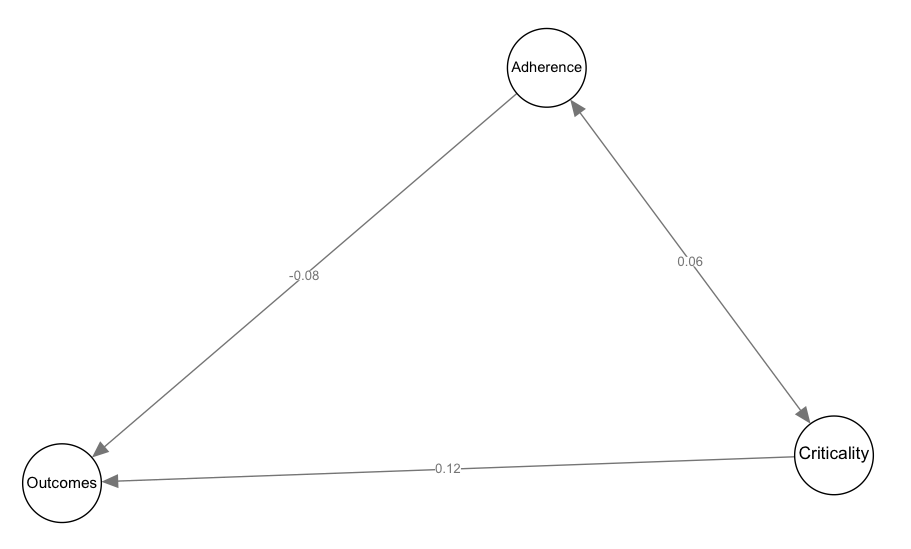
\includegraphics[width=\columnwidth]{modelzero}
	\caption{Model Constructs}
	\label{fig:model_constructs}
\end{figure}

\subsection{Situating the Constructs in Software Development}

To measure Outcomes, Adherence, and Criticality in the context of the software development lifecycle, we need to describe the components of software development in which vulnerabilities are introduced and found, to which security practices are applied, and by which the software may be attacked.   Vulnerabilities may not only be problems in code (`bugs'~\cite{mcgraw2006software}) but may also be, for example, design issues (`flaws'), documentation issues, and configuration issues. We define a set of vulnerability sources, based on the definition of vulnerability we have adopted(Section ~\ref{sec:model_contruct_outcome}):  
 \begin{itemize}
 	\item \textbf{Specification} - All activities, e.g. planning, preparation, requirements definition, and design that precede, chronologically or conceptually, coding. 
 	\item \textbf{Coding} - The development and maintenance of software features.
 	\item \textbf{Testing} - The quality assurance activities applied to developed software before it is released.
 	\item \textbf{Operations} - The configuration and use of the released software, and feedback from the software's users to the development organization.
 \end{itemize} 
The vulnerability locations may also be viewed chronologically, as development phases. Boehm ~\cite{boehm1981economics} reports that the earlier in the development process a defect is resolved, the cheaper it is to resolve. We can use data collected according to this scheme to analyze whether vulnerabilities follow the same cost pattern as defects. While many projects will have a more detailed set of development process phases, we conjecture that these phases are present in the majority of software development projects.

As a refinement of the basic constructs model from figure~\ref{fig:model_constructs}, we incorporate the phases into the construct model, as illustrated in \label{fig:model_constructs_phases}

\begin{figure}
	\includegraphics[width=\columnwidth]{PracticesDiagram}
	\caption{Model Constructs and Phases}
	\label{fig:model_constructs_phases}
\end{figure}


\subsection{The Security Practices Evaluation Framework}

To collect empirical data to test the constructs and their relationships, we have developed a data collection framework for the model, available online~\cite{morrison2016spefsite}.   We now present the data elements from the data collection framework. To ground the model and the present study, we include a hypothesis for each data element, which serves as both our reason for its inclusion in the framework and a testable component of the model. We collect Context Factors to measure Criticality, Practice Adherence Metrics to measure Adherence, and Outcome Measures to measure Outcomes.
\subsubsection{Context Factors}
\label{sec:model_cf}

Drawing conclusions from empirical studies in software engineering is difficult because the results of  any process largely depend upon the relevant context variables. One cannot assume a priori that a study’s results generalize beyond the specific environment in which it was conducted [5???]. Therefore, recording a study’s context factors is essential to understanding the generality and utility of the conclusions as well as the similarities and differences between the case study and one’s own environment. Dyba et al. ~\cite{dyba2012what} suggests the question `Does the inclusion of this information explain the constraints on, or the opportunities for, the phenomenon I am studying?' as a guide for including context factors. Jones~\cite{jones2000software} suggests six categories of measurements to be collected for every project; software classification, sociological, project-specific, ergonomic, technological, and international. SP-EF includes the following context factors:
\begin{itemize}
\item \textit{Language} – Language in which the software artifact being measured is written, e.g. Java, C, C++, Python, PHP. \textit{Hypothesis}: Because languages vary in how much access they provide to system memory and hardware, language choice influences security criticality.
\item \textit{Operating System} - Operating system(s) on which the software runs, e.g. Linux, Windows, iOS. \textit{Hypothesis}: Because operating systems vary in how much access they provide to system memory and hardware, and because they reduce an attacker’s effort by presenting a single interface to the population of machines they are available on (monoculture), operating system choice influences security criticality.
\item \textit{Domain} – A description of the software’s purpose, e.g. application, framework, utility. 
\textit{Hypothesis}: Because software domain influences who uses the software, what access to system resources the software has, and how often the software is run software domain influences security criticality.
\item \textit{Product Age} – Number of years since the software began development. 
\textit{Hypothesis}: Because attack and defense techniques for software change over time, product age influences software performance and software criticality.
\item \textit{Source Lines of Code (SLOC)} - Total number of source lines of code (no comments, no blanks) as counted, for example, by the cloc or SLOCCount utilities. 
\textit{Hypothesis}: Because each line of code is an opportunity to make a mistake,  and because code size correlates with other measures of software complexity~\cite{herraiz2009statistical},  SLOC is positively correlated with security criticality.
\item \textit{Churn} – Total number of SLOC added, deleted, or changed during the measurement time period. 
\textit{Hypothesis}: Because changed code is correlated with defects, and even single-line changes   can cause vulnerabilities, Churn is positively correlated with security criticality.
\item \textit{Team size} – Total number of unique individuals in each of the following roles: Manager, Developer, and Tester. \textit{Hypothesis}: Team size is beneficial in enabling appropriate time and effort invested in its requirements, design, implementation, review, testing and documentation activities. Team size is detrimental in terms of knowledge transfer and training requirements. Team size is positively correlated with practice adherence, and influences security outcomes. Through management awareness, security criticality influences Team size.
\item \textit{Team Location} – Team Location indicates whether the team is collocated or distributed. \textit{Hypothesis}: Because knowledge transfer and team cohesion are affected by team distribution, Team Location influences practice adherence.
\item \textit{Methodology} – Software development process approach used by team. \textit{Hypothesis}: Because the degree of effort put in to software process planning, documentation, and controls supports control over the delivered software and consumes team resources, Methodology influences practice adherence and security outcomes.
\item \textit{Number of Machines} - Number of machines is a count of how many machines on which the software is installed. The rise of botnets, networks of computers that can be centrally directed, has created a black market for their services.  In 2013, an hour of machine time on a botnet ranged from 2.5 – 12 US cents , and so the number of machines a piece of software runs on is a risk factor. \textit{Hypothesis}: Because economies of scale and monoculture work to the benefit of attackers as well as providers, Number of Machines is positively correlated with security criticality.
\item \textit{Number of Identities} - Number of identities is a count of how many individuals data are managed by the software.  In 2011, a personal identity could be bought (in groups of 1000) for 16 US cents  , and so the number of identities a piece of software manages is a risk factor. \textit{Hypothesis}: Because economies of scale work to the benefit of attackers as well as providers, Number of Identities is positively correlated with security criticality.
\item \textit{Confidentiality, Integrity, and Availability Requirement} (from CVSS) – The CVSS specification includes three data elements, one for each of Confidentiality, Integrity, and Availability, for indicating the security sensititivty of data. The values for each element are subjective assessments of the most sensitive data that passes through, or is kept by, the software under consideration for its Confidentiality (CR), Integrity (IR), and Availability (AR) requirements. \textit{Hypothesis}: Because CR, IR, and AR describe the security importance of the software, they are positively correlated with security criticality.
\item \textit{Source Code Avalability} – Source Code Availability indicates whether the software is proprietary or open source. \textit{Hypothesis}: Anderson [ref] showed that Source Code Availability influences security criticality and practice adherence in both positive and negative ways, depending on project specifics.
\end{itemize}

\subsubsection{Practice Adherence Metrics}
Researchers have empirically evaluated software development practices for their security benefits, for example, in requirements engineering~\cite{riaz2014hidden}, design patterns~\cite{uzunov2015comprehensive}, threat modeling~\cite{shostack2014threat}, static and dynamic analysis~\cite{austin2013comparison}, code review~\cite{meneely2014empirical}, testing~\cite{austin2013comparison}, and attack surface analysis~\cite{theisen2015approximating}.

Different projects are unlikely to use the same set of security practices, or to use a given security practice in exactly the same way. Project teams may adapt their methodology through adding and dropping practices to suit the requirements of their customers, their business and operational environments, and their awareness of trends in software development. Adherence metrics are a means of characterizing the degree to which a practice is used on a project. 
We have included subjective and objective metrics for measuring practice adherence. People are the driving force behind process and practices, and their views should be considered. We adopt four measures from UTAUT ~\cite{venkatesh2003user}, a model for the study of technology adoption, and add a fifth measure to support measurement of productivity: 
\begin{itemize}
\item \textit{Usage} - How often is this practice applied? \textit{Hypothesis}: Usage is a direct measure of the frequency of the use of a practice, positively correlated with practice adherence.
\item \textit{Ease Of Use} - How easy is this practice to use? \textit{Hypothesis}: Ease of Use is positively correlated with practice adherence.
\item \textit{Utility} - How much does this practice assist in providing security in the software under development? \textit{Hypothesis}: Utility is positively correlated with practice adherence.
\item \textit{Training} - How well trained is the project staff in the practices being used? \textit{Hypothesis}: Training is positively correlated with practice adherence.
\item \textit{Effort} - How much time, on average, does applying this practice take each time you apply it? \textit{Hypothesis}: Effort is a direct measure of practice adherence.
\end{itemize}
To support triangulation with subjective metrics, and support for studies where the team is unavailable, we define the following objective practice adherence metrics:
\begin{itemize}
\item \textit{Frequency}: Number of references to the practice, obtained by researcher observation and/or text mining. \textit{Hypothesis}:  How frequently practices are mentioned in project documentation and history is correlated with practice adherence.
\item \textit{Prevalence}: Proportion of the team applying the practice, the ratio of all practice users to all team members. \textit{Hypothesis}: Many studies, e.g. Venkatesh ~\cite{venkatesh2003user} and Witschey ~\cite{witschey2015quantifying}, show use by other team members to be correlated with why developers use practices. \textit{Hypothesis}: Prevalence is positively correlated with practice adherence.
\end{itemize}
For each security practice adherence event, we recorded the following data elements:
\begin{itemize}
\item \textit{Event Date} – Date on which document was created.
\item \textit{Practice} – Name of security practice associated with document. 
\item \textit{Source} – Data source for document. Possible Values: Version Control, Defect Tracker, Email.
\item \textit{Document Id} – Id of document in its source, e.g. commit hash, bug tracker id, email id.
\item \textit{Creator} – Author of the source document.
\item \textit{Assignee} – For defect report documents, the person assigned the defect, where applicable.
\end{itemize}

While the practice adherence metrics are not tied to a specific set of practices, we have defined a set of software development security practices, based on prior art. We read through the BSIMM, SDL, SAFECode, and OWASP practice lists, filling out the practice adherence template (\ref{sec:model_contruct_adherence}) for each security practice. We identifying 16 practices that, in combination with roles (e.g. Manager, Developer), verbs (e.g. ‘implement’, ‘test’, ‘document’) , phases (e.g. ‘Design’, ‘Testing’), and artifacts (e.g. ‘Requirements’, ‘Source Code’, ‘Regulations’), were sufficient to classify the source practices we identified. We excluded three of the practices, ‘Apply Security Principles’,  ‘Monitor Security Metrics’ and ‘Publish Disclosure Policy’ from the framework because they were mentioned less than 2\% of the time across our sources.
Once we had classified the practices, we revisited the text of the source practices, and extracted representative keywords and questions characterizing how the practice is implemented. 
 Table 1 lists the practices, with descriptions, and keywords for each practice. Documentation for all of the roles, verbs, phases, artifacts, keywords, and questions is available at the website~\cite{morrison2016spefsite}.

\subsubsection{Outcome Measures}
In this section, we describe the set of attributes and values that are used to describe the security-related outcomes of the project. 

While hundreds of security metrics have been proposed~\cite{rudolph2012critical},~\cite{verendel2009quantified}, tracking a relatively small set of attributes for each vulnerability detected in the software is sufficient to replicate many of them. In addition to data kept for defects (e.g. those attributes listed by Lamkanfi et al.  ~\cite{lamkanfi2013eclipse}), we collect:
\begin{itemize}
\item \textit{Source} – The name of the bug tracker or bug-tracking database where the vulnerability is recorded.
\item \textit{Identifier} – The unique identifier of the vulnerability in its source database.
\item \textit{Description} – Text description of the vulnerability.
\item \textit{Discovery Date} – Date the vulnerability was discovered. 
\item \textit{Creation Date} – Date the tracking record was created.
\item \textit{Patch Date} – The date the change resolving the vulnerability was made.
\item \textit{Release Date} – The date the software containing the vulnerability was released.
\item \textit{Severity} – The criticality of the vulnerability. 
\item \textit{Phase}  – Indication of when during the development lifecycle the vulnerability was discovered
\item \textit{Reporter} – Indication of who found the vulnerability. (Optional) Role Name and/or email address of person in the reporter role. 
\end{itemize}

Given a collection of vulnerabilities with the attributes specified above, we can compute the following measures:
\begin{itemize}
\item \textit{Pre-release Vulnerabilities} - Vulnerabilities found in new and changed code before software is released. \textit{Hypothesis}: The goal of security practice adherence is to avoid releasing software with vulnerabilities, so pre-release vulnerabilities are positively correlated with security effort, and negatively correlated with security outcomes.
\item \textit{Post-release Vulnerabilities} - Vulnerabilities found in new and changed code after software is released. \textit{Hypothesis}: Post-release Vulnerabilities represent a failure of the process to catch vulnerabilities pre-release, and are negatively correlated with security outcomes.
\item \textit{Vulnerability Density} - Vulnerability Density (Vdensity) is the cumulative vulnerability count per unit size of code ~\cite{alhazmi2007assessing}. We adopt a size unit of thousand source lines of code (KSLOC). \textit{Hypothesis}: Vulnerability Density is a derived measure negatively correlated with security outcomes ~\cite{alhazmi2007measuring}.
\item \textit{Vulnerability Removal Effectiveness} - Vulnerability Removal Effectiveness (VRE) is the ratio of pre-release vulnerabilities to total vulnerabilities found, pre- and post-release, analogous to defect removal effectiveness ~\cite{kan2002metrics}. Ideally, a development team will find all vulnerabilities before the software is shipped.  VRE is a measure for how effective the team’s security practices are at finding vulnerabilities before release. \textit{Hypothesis}: VRE is positively correlated with practice adherence, and negatively correlated with security outcomes.
\end{itemize}


\subsection{Putting it all together; Linking SPEF to the Model}

Figure X-marks-the-full-model-spot presents the model, annotated with each SPEF data element in its hypothesized relationship to the model. 
In this section, we build three graphical models of the hypothesized relationships described above, representing three levels of measurement detail.





\section{Methodology}
\label{sec:methodology}
In this section, we present the steps required for analyzing a data set in terms of the security outcomes theoretical model.

\subsection{Subject Selection}
Select a dataset containing measurements of variables that can be related to the structural model's Asset Risk, Software Risk, Adherence, and Outcomes constructs.  

\subsection{Link data source variables to model constructs}
Use theoretical relationships to link measurement model data source variables to structural model constructs. Consider each variable in the dataset, and assign eligible variables to the appropriate model construct, per the model construct definitions and the variable listed in \ref{tab:model_spef_metrics}. For example, if the dataset contains a code churn metric, associate it with Software Risk. 

\subsection{Evaluate collected data for fit problems}
Standard SEM approaches assume linear relationships between variables in both structural and measurement models, requiring researchers to pre-examine the data for non-linear relationships. Potential solutions where nonlinear data is found include excluding outliers and adding appropriate power terms.

As SEM solves for the covariance or correlation of variables with each other, SEM depends on the variances of the measured variables to be within an order of magnitude of each other, and typically in the range of 1$-$10. Transform high-variance variables, by taking their logs, or square roots, or by standardizing them. In this work, where a measured variable variance exceeds the variances of other measured variables by an order of magnitude or more, we create a transformed variable taking the log of the sum of the original variable value and a small constant, 1. For example, lines of code varies widely, and  we transform logSLOC = (total\_code\_lines+1).

Collinearity between measurement variables affects model fit. We check for collinearity between measurement variables in the dataset, and drop collinear variables (as measured by a Spearman correlation coefficient greater than 0.7) that are theoretical alternatives. For example total\_contributor\_count and TeamSize are collinear in the CII dataset, and we choose logContributorCount to represent the concept.

\subsection{Estimate SEM model} 
The specified relationships in the structural and measurement models represent a system of equations. SEM software is written to solve these systems of equations. In this work, we apply lavaan.  Encode the combined structural and measurement models in a SEM modeling tool, and run the tool to obtain estimates for the model. 

\subsection{Model Fit}
% TODO [Paragraph explaining model fit and indicators]
Once a set of estimates has been generated for a given model and dataset, SEM users evaluate fit measures and residuals to assess the suitability of the model. Model fit indicators and residuals both represent the degree of misfit between the model and the dataset. 

No single SEM fit measure captures all of the diagnostic information available, so SEM theorists and practitioners recommend reporting multiple goodness-of-fit and badness of fit measures.
The model fit measures recommended by Kline~\cite{kline2015principles} are as follows:
\begin{itemize}
	\item Model chi-square with degrees of freedom and p-value. Ratio of 3 or less for chi-square to degrees of freedom indicates acceptable fit.
	\item Stieger-Lind Root Mean Square Error of Approximation (RMSEA) - RMSEA is a `badness-of-fit' measure, where values less than 0.10 indicate acceptable fit.
	\item Bentler Comparative Fit Index (CFI) - CFI compares fit of the researcher's model to a baseline model, where values of 0.90 or greater are viewed as acceptable fit.
	\item Standardized Root Mean Square Residual (SRMR) - SRMR is a `badness-of-fit' measure of the difference between the observed and predicted correlations. Zero is a perfect score, scores below 0.08 are viewed as sufficient.
\end{itemize}

\subsection{Re-specification}
Kline~\cite{kline2015principles} and Loehlin ~\cite{loehlin2004principles} both offer methodologies for diagnosing fit problems and revising the data and the model in principled ways. We present a set of steps derived from these sources for application to our data and measurement model. We declare alterations to the structural model out of scope for the present work, as the work is intended to assess our structural model. 

If model fit indicators show poor fit between the data and the model, consider adding, dropping, or moving measurement variables, if theory supports doing so. In the present study, we do not alter the constructs or relationships in the structural model, but we do allow a list of transformations for the measurement model, as follows:
\begin{itemize}
	\item SEM requires measurement model variable variances to be within a narrow range of each other. Transforming a variable by taking its log, square root, or multiplying by a constant is at the discretion of the researcher (transformation must be documented).
	\item Choice of measurement variable to construct association is at the discretion of the researcher. 
	\item Where more than one measurement variable measures the same concept (e.g. team size measured by a count and by an ordinal variable), variable choice is at the discretion of the researcher. 
\end{itemize} 

If transforming the data does not yield adequate fit, the next step is to evaluate the measurement model. Loehlin~\cite{loehlin2004latent} recommends, as a first step for respecification,  fitting the data to a model in which the latent variables are completely intercorrelated, yielding a perfectly fitting structural model, and revealing fit difficulties rooted in the measurement model. 

In addition to the global fit indicators presented above, researchers must examine residuals to assess local model fit. Residuals, also called error terms, are associated with each measurement variable, and represent variance not explained by the construct with which the measurement is associated. Residual values near zero indicate that the construct accounts for the bulk of the variance in the measurement variable. Residual values near one indicate that the construct does not account for the bulk of the variance in the measurement variable, and should prompt investigation, re-specification, and/or explanation. Residual values provide a diagnostic of model fit.

\subsection{Report Results}
% See page 464 of Kline for details
Kline~\cite{kline2015principles} recommends reporting model fit in the terms of the global fit indicators, and in terms of comparison between the expected theoretical relationships embedded in the model and the actual parameter magnitudes and signs observed in the data. In this work, we apply basic interpretations, focusing only on the sign and relative magnitude of each parameter estimate, as compared to our theorized expectations, where sign indicates direction of influence, and magnitude indicates effect size. For the parameter estimates of measurement variables associated with a single latent variable, sign indicates direction of influence, and (standardized) parameter estimates indicate the relative importance of each measurement variable's effect on the latent variable. For latent variable relationships, sign indicates the direction of influence, and magnitude indicate the relative importance of the latent variable's effect on the receiving latent variable, as compared with the magnitude of the other latent variable parameter estimates.
\section{Evaluation}
\label{sec:evaluation}

We evaluated our model in two ways; at the construct level through applying structural equation modeling to a dataset of projects for which security is a concern, and at the SPEF framework level by conducting two case studies of open source development projects, examining the effects of security practice use on security outcomes. In this section, we present a summary description of our case study protocol, SP-EF, and how we apply it to our data collection and analysis. SP-EF and all study artifacts are available online ~\cite{morrison2016spef}. 

\subsection{Quantitative Study Methodology}

To quantitatively assess the relationships between constructs in our proposed model, we applied Structural Equation Modeling~\cite{kline2015principles} to the Core Infrastructure Initiative~\cite{lf2016cii} (CII) census dataset (~\footnote{\url{https://github.com/linuxfoundation/cii-census}}). 

\subsubsection{Structural Equation Modeling}

Kline~\cite{kline2015principles} emphasizes that the point of SEM is to test a theory by specifying a model that represents predictions of that theory among plausible constructs measured with appropriate observed variables (those that can be directly measured). Latent variables represent plausible constructs, e.g. ‘intelligence’, or ‘Criticality’, that cannot be directly measured, but that can be indirectly measured in terms of one or more observed variables. SEM is often applied in psychology and education, to build a measurement model for the constructs measured, and to allow assessment of how well measurement instruments test the constructs measured. 

SEM studies are organized around six steps: specification, identification, data selection and collection, estimation, re-specification, and reporting. In model specification, researchers express the hypothesized relationships between observed variables and latent variables, typically in the form of a graphical model. Each edge in the graph represents a parameter to be estimated, indicating the strength of the relationship between the nodes connected by the edge. In identification, the specified model is checked against statistical theory for whether all of the model’s parameters can be estimated. If the original model cannot be identified, it must be revised in light of both statistical theory and the theory the researcher is expressing in the model. In data selection and collection, data for each of the model’s observed variables is chosen, and collected. In estimation, the observed data and the model are checked for fit.  If appropriate fit is achieved, the parameter estimates can be interpreted for implications of the theorized relationships and the observed data. If appropriate fit is not achieved, the list of model changes developed during specification should be considered in re-specifying the model.  When reporting the results of SEM studies, the model, parameter estimates, and fit measures should be included in the report.
Examples of SEM use in software engineering and information technology include Capra et al.~\cite{capra2008empirical}, Wallace and Sheetz~\cite{wallace2014adoption}, and Gopal et al.~\cite{gopal2005impact}.

\subsubsection{Specification}
For causal hypotheses, we used the hypotheses for each construct in Section \ref{sec:model} to create edges in the model specifying each element’s effect on security risk, practice adherence, and security outcomes.  We model security risk, security effort, and security outcomes as latent variables, explanatory entities that reflect a continuum that is not directly observable~\cite{kline2015principles}. In SEM, latent variables are represented in diagrams as ovals or circles.

\subsubsection{Identification}
In identification, the specified model is checked against statistical theory for whether all of the models parameters can be estimated. Identification is analogous to checking whether a set of equations is solvable given their structure and the data at hand.  Our construct model contains no feedback loops making it both recursive, and, therefore, identified, by Rule 7.1 of Kline ~\cite{kline2015principles}.  

\subsubsection{Data selection and collection}

Kline ~\cite{kline2015principles} states that SEM is a large-sample technique, reporting median sample size in the literature of 200 cases.  Factors that drive the need for a large sample include the size and complexity of the model to be estimated, non-normally distributed data, categorical data, and imprecisely measured data. To obtain a sufficient sample, we draw our study data from summaries of repository data. In particular, we chose the CII census dataset
	because: collects a subset of our constructs, 
We applied the Boa [44] language infrastructure to the full September 2015 Github dataset ro collect project summaries for 68,035 Java language projects We operationalize practice adherence by counting references to each practice’s keywords in commit messages. 

To identify a practice, we adapt Ernst and Mylopoulos’s [28] technique of labeling events in project history, though we measure security practice use rather than requirements discussions, and we use the SP-EF keywords, listed in Table 1, rather than drawing from the ISO 9126 quality model. 

We developed a Boa job  that scans Boa datasets for projects, and produces a single-line summary for each project, including the project name, url, Source Lines of Code (SLOC), number of developers (Devs), references to ‘CVE-‘ records, and keyword counts for each of the security practices and the ‘Security-Related’ keywords.  

To exclude toy projects, we limited the results to those projects with two or more developers, and 1000 or more lines of code.  Because Boa only stores source code information for Java projects, our results include only Java projects. We operationalize security outcomes by counting references to CVE’s in commit messages.  We identified 121 unique projects with one or more CVE’s. 

We randomly sampled 121 projects with no CVE’s from the remaining projects to form a data set of 242 projects.
We were not able to obtain all SP-EF measurements from the repositories. 

To compensate, we kept the structural model intact and adapted or removed some elements of the measurement model to account for the data available from our data sources. 

We now list the adaptations. Since all projects are written in Java, we elided language from the model. 

We removed domain, number of identities, CR, IR, and AR because any selection process we could develop to set values for the variables would add noise to the data. Because of the nature of commit logs, we assume that each unique email address associated with the commit is for a developer. We use the number of developers (‘Devs’), as a proxy for team size. As a proxy for number of machines, we used the number of Google  search results for each repository, reasoning that the search result counts – how widely known the project is - is proportional to how widely used the project is We use counts of CVE references as a proxy for total public vulnerabilities (pre- and post-release), and we calculate VDensity. We do not have a breakdown of when vulnerabilities were discovered for each project, and so we do not measure Pre-Release Vulnerabilities, Post-Release Vulnerabilities, and we do not calculate their ratio, VRE. We use the CVE count and VDensity as our measures of security outcomes. 



\subsubsection{Estimation}
\subsubsection{Re-specification}
\subsubsection{Reporting}


\subsection{Qualitative Case Study Methodology}
In this section, we present a summary description of our case study protocol, SP-EF, and how we apply it to our data collection and analysis. SP-EF and all study artifacts are available online ~\cite{morrison2016spef}. 

Williams et al. ~\cite{williams2004toward} proposed the Extreme Programming Evaluation Framework (XP-EF), a set of repeatable measures for assessing the degree to which a team held to XP practices enabling replication and meta-analysis of studies. We emulate the organization and intent of XP-EF in the construction of SP-EF, while adapting the content to focus on security practice adherence rather than Extreme Programming. SP-EF provides guidelines for data collection of context factors, practice adherence metrics, and outcome measures. Context factors characterize the project by, for example, its size and purpose. Practice adherence metrics are a means of characterizing the degree to which a practice is used on a project. SP-EF includes objective and subjective metrics for measuring practice adherence. Outcome measures characterize the software's security performance. Table \ref{tab:paComparisonTable} lists the SP-EF practices.  
% \ref{fig:fig_context} presents an overview of the SP-EF practices and their place in the software development lifecycle.

%\begin{figure*}
%	\includegraphics[width=7in]{figure/PracticesDiagram.png}
%	\caption{SP-EF Software Development Security Practices}
%	\label{fig:fig_practices}
%\end{figure*}

To assess our data collection methods and to increase confidence in our findings, we triangulate, collecting data in three ways; through qualitative observation, survey, and text mining of the team's issue tracker. We worked with the project staff and read through the project documentation for qualitative evidence of the security practices, based on the SP-EF subjective practice adherence measures. We conducted a survey of the team, using the SP-EF practice adherence survey. The survey contains demographic questions (e.g. role, time on project), four questions aligned with the SP-EF subjective measures for each SP-EF security practice, and open-ended questions allowing survey participants to express their views. Each of the four subjective adherence measures are actionable; comparing observed results with expected results can be translated to actions for each measure in the following ways;
\begin{itemize}
	\item Usage - ``How often is this practice applied?'' - Lower than expected usage can be addressed by discussing, or requiring, higher frequency of use with the team.
	\item Ease Of Use -``This practice is easy to use'' - Lower than expected Ease of Use can be addressed through, for example, examination and refactoring of work practices, and through training.
	\item Utility - ``This practice assists in preventing or removing security vulnerabilities in our product'' - Lower than expected Utility can be addressed through examining practice use, and, possibly, discontinuing use of the practice.
	\item Training - ``I have been trained in the use of this practice'' - Low training for a practice can be addressed through increasing the availability of training.
\end{itemize}

We piloted the survey within the research group, and with researchers at two companies. The survey questionnaire is available from the SP-EF website. We obtained objective SP-EF practice adherence measures for the team by applying a basic text mining technique, keyword counting, to the project's issue tracking records. The text mining classification procedure is available as an R package, linked from the SPEF website~\cite{morrison2016spef}.   To develop an oracle for assessing the performance of the text mining, we read and classified the set of issue tracking records described above according to the guidelines for identifying the presence of SP-EF practices. We compute recall and precision for the mined objective measures, compared to the manual oracle. 

\subsection{Subject Selection}
We select projects for this study based upon meeting the following criteria:
\begin{itemize}
	
	\item Available records of software security vulnerabilities
	\item Version control system access, providing both project source code and the history of changes to the code over time
	\item Bug tracker system access, providing records of vulnerability and defect discovery and resolution
	\item Project documentation, providing access to information about the project’s development process and practices
\end{itemize}

We collect project documentation and history using the project’s website, version control system, and bug tracker, as primary sources, and as sources for links to further information. 

For this study, we chose OpenSSL, to evaluate security practice use before and after the Heartbleed bug.  For comparison across cases, we choose phpMyAdmin, an open source project of similar age and size to OpenSSL, allowing comparison of how security practices and outcomes are similar and different between the projects. 

\subsection{Data Collection}

We collect data through qualitative observation and text mining of the team's emails, issue tracker, and commit messages. We read through the project documentation for qualitative evidence of the security practices, based on the SP-EF subjective practice adherence measures. We obtained objective SP-EF practice adherence measures for the team by applying a basic text mining technique, keyword counting, to the project's issue tracking records. The text mining classification procedure is available as an R package, linked from the SP-EF website~\cite{morrison2016spef}.   To develop an oracle for assessing the performance of the text mining, we read and classified a subset of the emails, issue tracking records, and commit messages described above according to the guidelines for identifying the presence of SP-EF practices. 

For each practice, we used the search strings listed in the ‘Keywords’ column of Table 1, and recorded each instance of practice use.  We collected data by two means:
\begin{itemize}
	\item We used a script, available from the SP-EF website, to iterate over each commit, issue, and email, and generate security practice event classifications.
	\item The first author manually examined each project for security practice use and generated security practice event classifications. Additional raters classified a randomly selected pool of issues, and we compared their results to the automated classifications.
\end{itemize}

For each artifact we identified, we recorded the document name, URL, age, and made note of any available change history, e.g. wiki page change records. We manually classified pre- and post-release vulnerabilities based on a study of who reported the vulnerability and whether they were identifiable as a project member.

\subsection{Analysis}

We qualitatively compare pre-security event data with post-security event data for each project, looking for changes in the security practices selected by the team, and changes in frequency of use of the practices by the team. In the case of OpenSSL, we manually classified 500 commits, bug tracking issues, and emails from the year before April 1, 2014 (Heartbleed), and 500 more from the year ending April 1, 2016.  We chose the earlier time period to reflect pre-Heartbleed efforts, and the more recent time period to reflect ongoing practice rather than the immediate response to Heartbleed. In the case of phpMyAdmin, we chose the year 2007, reflecting phpMyAdmin data before its participation in GSOC, and from the year ending April 1, 2016, reflecting current practice. By comparing the data sets, we expect to find security-focused practice changes in the text of the sets of project data.

To evaluate RQ1, we collect frequency metrics through manual review of each project’s artifacts; project documentation, project emails, bug tracking issues, and commit messages.  

To evaluate RQ2, we track two outcome measures, counts of CVE and Security-Related (SR) events. CVE's are publicly reported vulnerability counts, which may understate the total vulnerability count.  SR events are counts of references to a set of keyword that represent those found in typical discussions of security, acting as a proxy for the team's awareness of security. Lower values for CVE and SR may indicate high code quality and/or opportunities for discovering latent vulnerabilities. We examine the relationship between our practice adherence metrics and CVE and SR.

\section{Discussion}
\label{sec:discussion}

In this section, we compare our expectations and findings across our case study results, and discuss the implications for our method, model, and data.

%	actual(expected)magnitude*statsig
%		== signs 'as hypothesized'
%		
%			NVD				CII
%	AR-SO	+(+)0.05*		-(+)0.14*
%	SR-SO	+(+)0.12*		+(+)0.28*
%	PA-SR	+(-)0.78*		-(-)0.44
Asset Impact positively (NVD, as hypothesized) and negatively (CII, contrary to hypothesis) affected Outcomes, and was statistically significant in both the NVD and CII datasets. The 0.14 magnitude in the CII dataset was roughly triple the 0.05 magnitude in the NVD dataset. We attribute the magnitude difference primarily to the different metrics used to assess Software Risk in each dataset. Asset Impact was proportionally smaller than Software Risk for both datasets. The data available in the NVD and CII datasets are a subset of the metrics we expect to influence Asset Impact, and both datasets are constrained to a subset of software projects, by construction. We conjecture that more accurate asset data, as well as a broader selection of projects, would affect the proportion of Asset Impact. In the case of CII's Asset Impact being negatively associated with Outcomes, we observe that the sole measure of CII Asset Impact is package popularity, an indicator within the Debian ecosystem of the number of systems with that package installed. While in the present case, running on more machines is associated with fewer vulnerabilities, contrary to our hypothesis, the effect may be an illustration of Eric Raymond's 'many eyes make all bugs shallow', as measured by the number of eyeballs of users of the software. A number of studies have examined Linus' law in the context of developer attention (e.g. ~\cite{meneely2013when}) rather than user attention, as measured here. 

Software Risk, as hypothesized, positively affected Outcomes, and was statistically significant, in both the NVD and CII datasets. The 0.28 magnitude in the CII dataset was roughly double the 0.12 magnitude in the NVD dataset. We attribute the magnitude difference primarily to the different metrics used to assess Software Risk in each dataset. We conjecture that the metrics available in each dataset are of value for assessing Software Risk.  Of particular note are the network risk metrics each dataset provides. Both NVD cvss\_access\_vector and the similar CII direct\_network\_exposure metrics were statistically significant contributors to Software Risk. A Software Risk-related implication of our study is that existing measures, particularly number of developers and SLOC, capture Outcome-related effects on software. Larger projects, as measured by team size and code size, are more likely to have CVE's reported against them. While not a new finding, our data and model are in agreement with prior research~\cite{shin2011evaluating,meneely2013when}.

Adherence positively (NVD, contrary to hypothesis) and negatively (CII, as hypothesized) affected Software Risk, and was statistically significant in the NVD dataset. The 0.78 magnitude in the NVD dataset was roughly double the magnitude in the CII dataset, again something we attribute to the different metrics used to assess Adherence in each dataset. Our NVD data did not confirm Kaminsky's hypothesis that software quality is improving over time, with our adherence-over-time measure increasing Software Risk. Our Our CII data did not contain a similar metric. However, we observed several counter-trends in the underlying NVD data. We observed an improvement in CVSS Authentication Risk (Figure \ref{fig:nvd_cvss_auth}). On average, vulnerabilities are requiring more authentications over time, implying that development teams are putting an increasing amount of functionality behind access control. One implication of our study is the evident need to collect and evaluate a set of adherence metrics for assessing Adherence and its effects on mitigating Software Risk.

The datasets we studied did not contain a complete set of the measurement model metrics we are interested in, as listed in Table \ref{tab:model_spef_metrics}. For the metrics the datasets did contain, we found statistically significant support for each of them, with the exceptions of process\_network\_data, potential\_privilege\_escalation, Code Comments, and Website Risk from CII. 

For the structural model, while our current evidence for the constructs and their relationships is, in part, equivocal, we have a set of conjectures and the data they require, to establish whether we can retain the model. 

We view our contributions in this work to be the following:
\begin{itemize}
	\item A proposed model of the constructs affecting software development security outcomes
	\item A proposed set of metrics to measure for assessing security posture in software development
	\item Empirical evaluation of the proposed model and metrics using two open source datasets
	\item A process for revising the model and metrics, supported by SEM for statistical analysis of model and metric fit. 
\end{itemize}	

Stepping back from the details of the case study measurements, we can use the current model, its estimates, and its residuals, as a baseline for where we stand in terms of measuring the effects of multiple constructs on security outcomes in software development. In particular, we can use the model as 'straw man' for evaluating alternative constructs affecting software security outcomes, we can use the parameter estimates as to assess the relative effects of the constructs we measure, and we can use the residuals as a guide to improving measurement of the constructs we choose. 

We opened the paper with the example of Cloudbleed, illustrating the need to assess software context as well as software quality. We have built a modeling process, identified metrics to collect, collected data, and analyzed the data, supporting the notion that Asset Impact is a component of security Outcomes, in addition to Software Risk. Further development of the model and its constructs, and the metrics and their measurement and collection should provide further insight into the software development and usage constructs affecting security outcomes for the software's developers, managers, and users.
\section{Limitations}
\label{sec:limitations}

We now discuss threats to validity of our study.

Our two datasets represent thousands of open source and commercial software projects. However, each dataset represents a restricted subset of software development projects, where the NVD dataset is constrained to projects with CVE records, and the OpenHub dataset is constrained to open source projects as chosen by the site's administrators. Our results are constrained to open source projects reported on by OpenHub that also have vulnerabilities reported in the NVD. Generalizing to proprietary projects, and to projects that have security vulnerabilities reported by other means, and to projects that do not have vulnerabilities will require alternate data sources.     

Kaminsky~\cite{kaminsky2011showing} critiqued the NVD data, pointing out that the existence of a vulnerability record is more indicative of reporter and finder interest in the software than of the software's quality. The strength of the effect of user\_count on Outcome shown in our analysis offers empirical evidence for Kaminsky's concern. We view reporter and finder interest as indicative of the kind of usage risk we seek to measure, distinct from software quality. Further work comparing software quality between samples of non-NVD projects and NVD projects is needed to establish the strength of the effect of reporter and finder interest, and its effect on usage risk. 

Use of the NVD vulnerability counts is a limitation, as they are externally reported and may understate the presence of security issues. Where software development teams track vulnerabilities and related security issues internally, that data can be used to increase the model's accuracy.

The variety of factors involved in security measurement suggest that further investigation is necessary. Complete validation of the model would require use of a variety of frameworks, metrics, and data sources to evaluate the constructs and their relationships. That said, we used two independent data sources, increasing confidence in correlations found in the data sets. 

In terms of construct validity, we propose a structural model of factors we believe to be relevant, and a measurement model based on the literature, but we leave room for augmenting the existing set of factors and the measurements taken on those factors. The analytical tools of SEM provide diagnostics to check for residual error and modification potential, enabling iteration over the structural and measurement models to account for additional factors in the model. 
%[Add refs to Mell/Scarfone Improving CVSS and An Analysis of CVSS scoring, add discussion of limits of NVD use of web forms for reporting vulns/cvss.]
  
The two datasets we used each contain subsets of the variables we theorize are necessary to assess security posture. We expect that the missing variables influence both the relative measures of each factor, and of the relationships between each factor. 

Statistical model-building in software engineering often uses Bayesian Belief Networks rather than SEM, e.g. Fenton~\cite{fenton2012risk}. Judea Pearl has claimed the two techniques are essentially identical, preferring SEM when the research question if of the form `What factors determine the value of this variable?' - \footnote{\url{http://causality.cs.ucla.edu/blog/index.php/2012/12/07/on-structural-equations-versus-causal-bayes-networks/}} We view our task in terms of determining the factors behind the values of the modeled variables, leading us to cast the model in terms of SEM.
\section{Conclusion}
\label{sec:conclusion}

In this paper, we have presented a model of factors affecting software security, with empirical tests of the model using two datasets. Our results indicate that:
\begin{itemize}
	\item
\end{itemize} 	
These findings correlate with previous findings by X, Y, and Z.

Our data suggest that not only software attributes, but the context of software use must be accounted for to assess the state of software security. Researchers and practitioners should measure both software attributes and software usage context when assessing software development practice adherence. That said, our analysis shows correlation, but not causation. Further work including manipulation of variables must be conducted to assess the causes of software insecurity and security. 

\section{Acknowledgements}

This work was supported through an IBM PhD Fellowship, and the USA National Security Agency (NSA) Science of Security Lablet. Any opinions expressed in this material are those of the author(s) and do not necessarily reflect the views of IBM or the NSA. We would like to thank the North Carolina State University Realsearch group for their helpful comments on the paper.






%\input{samplebody-conf}

\bibliographystyle{ACM-Reference-Format}
\bibliography{modeling} 

\end{document}
